\documentclass[12pt,a4paper,UKenglish]{article}
\usepackage[utf8]{inputenc}
\usepackage[T1]{fontenc, url}
\usepackage{float}
\usepackage{graphicx}
\usepackage{babel,csquotes,newcent,textcomp}
\usepackage[backend=biber,sortcites]{biblatex}
%\usepackage{subfig}
\usepackage{hyperref}
\hypersetup{colorlinks=true, linktoc=all, linkcolor=blue,}



\title{Preliminary report on master project}
\author{Rikesh Chauhan}
\date{}

\addbibresource{pre.bib}

\begin{document}
\maketitle

\section{Introduction}
This report is a brief overview of my master project on wireless power transfer through inductive coupling. It is the documentation of the schematic of complete design of the power receiving unit. It includes brief explanations about choice made. Figure \ref{fig:blockd} is the block diagram of the design.

\begin{figure}[htbp] %figure placement: here, top, bottom, or page
   \centering
   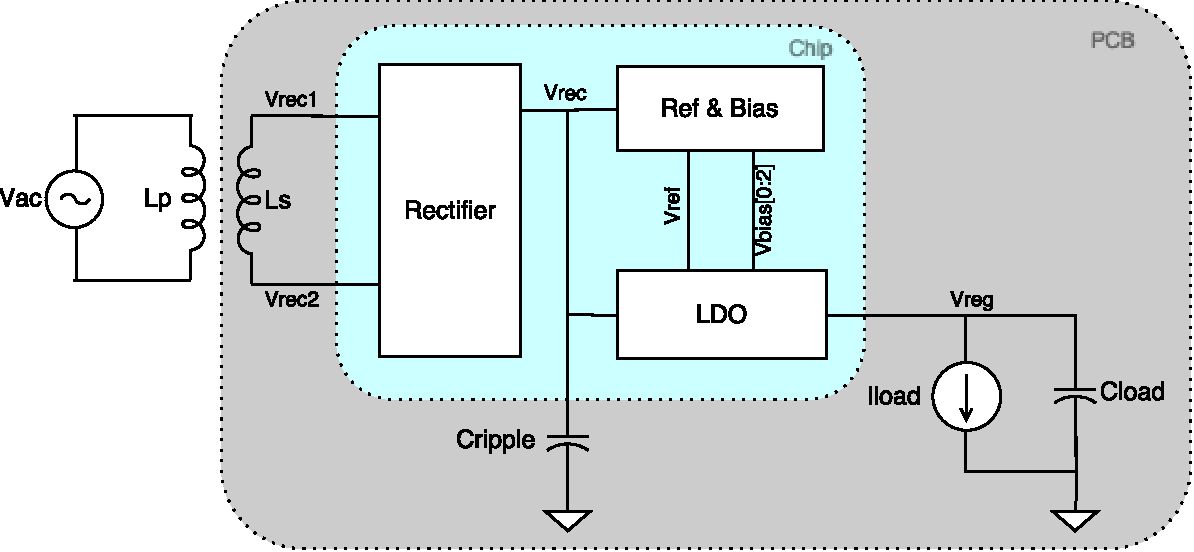
\includegraphics[width=\textwidth]{img/block_diagram.pdf} 
   \caption{Block diagram of complete design}
   \label{fig:blockd}
\end{figure}

As shown in the block diagram above, the design includes inductors, rectifier, LDO and reference and biasing circuits. The following is the design discussion of each sub circuits.

\section{Rectifier}

The most basic rectifier is  the conventional full wave bridge structure where the diodes are replaced by the diode connected MOS devices in CMOS technology. This topology though being simple to implement, it has a major drawback. It requires at least twice the threshold of a MOS device as there are two diode connected MOSes in the conduction path for each cycle of the input signal.  

Gate cross coupled and fully gate cross coupled topologies are improvements over conventional full wave rectifier. In gate cross coupled rectifier, two diodes of conventional rectifier is replaced by two gate cross coupled MOSes working as switches where is voltage drop for every cycle is reduced to one threshold. Similarly, in the fully cross coupled rectifier, all diodes are replaced by switches and hence the voltage drop is further reduced to twice the conduction drop for every cycle. Even though this topology has least voltage drop, it suffers from the problem of reverse charge leakage when the input voltage is less than the output voltage.

All the above discussed topology suffer from either large voltage drop or large power loss because of which their use are limited in low power and low voltage devices. The popular techniques for higher efficiency are using gate cross coupled rectifier along with passive or active circuitry  for controlling other two pass devices. In passive rectifier, additional circuitry including bootstrap capacitor are used to reduce or eliminate threshold voltage one of which is discussed in this paper \cite{rectboot}. However, use of on-chip bootstrap capacitors limits it use where chip area and speed is of importance. On the other hand, in active rectifier, active circuitry is used control pass devices. The use of active circuitry increase both VCE and PCE because the pass devices are made to conduct in linear region and hence less conduction drop, and reverse current flow can be completely eliminated and hence less power loss. However active rectifier is not problem free either. The major issue is starting of the active circuit as there is no regulated supply at the start up. Active rectifier is chosen for this project, primarily for better VCE and PCE and secondarily to avoid the use large on chip capacitors \cite{rectrcc}  and \cite{rectcomp}.

\newpage
\printbibliography
\end{document}
